\documentclass{article}
\usepackage{fullpage}
\usepackage{amsmath}
\usepackage{verbatim}
\usepackage{graphicx}

\date{October 19, 2010}
\author{Matt Mosby}
\title{Creating Scaling Problem Domains for PFEM3d}

\begin{document}
\maketitle

\section{Introduction/Motivation}
In order to properly benchmark parallel codes, scaling tests must be
preformed to guage how well they will perform on large distributed
systems. PFEM3d uses MPI to solve large systems on distributed
systems, and we wish to guage how well it will perform on massively
parallel systems so that we may write proposals for computer time.
There are two predominant ways to test the scalability of a parallel
program: fix the problem size and increase the number of processors
used to solve (commonly called a fixed problem scaling test), or scale
the problem size proportionally to the number of processors used to solve
(commonly called the scaling problem scalability test). This document
outlines the procedure for creating computational domains for doing
the scaling problem scalability tests.

\section{T3dScale}
A small program has been written to create a computational domain to
solve which consists of smaller identical domains for each processor.
This program is called T3dScale. It reads a T3d mesh and a specially
flagged T3d input file and outputs a mesh for a distributed domain in
a cubic shape.  The following subsections outline the proper
formatting of the T3d input file, how files should be named, available
options, and other useful infromation.

\subsection{Formating the T3d Input File}
Of utmost importance is the following: {\bf The computational domain
  for each processor,} {\it i.e.} {\bf the mesh generated from this file,
  MUST be periodic and rectangular cubic!} Rectangular prisms may
work, but it has not been tested and there are no plans to extend
T3dScale to work with domains other than rectangular-cubics.

Thus the boundaries of the domain must be made rectangular-cubic and
periodic (using mirror).  Additionally, the boundary surface must be a
patch (surfaces are not yet supported, and due to the possibility of
having curved surfaces, they may never be).  Finally, the domain
boundary elements must be numbered according to figure \ref{fig:numbering}.  The actual
numbers may not matter so long as they are still numbered in the same
order, but this has not been tested.  The faces are numbers as
follows: vertical faces starting from x+ going CCW around the domain,
horizontal faces starting from z-.

\begin{figure}
\center
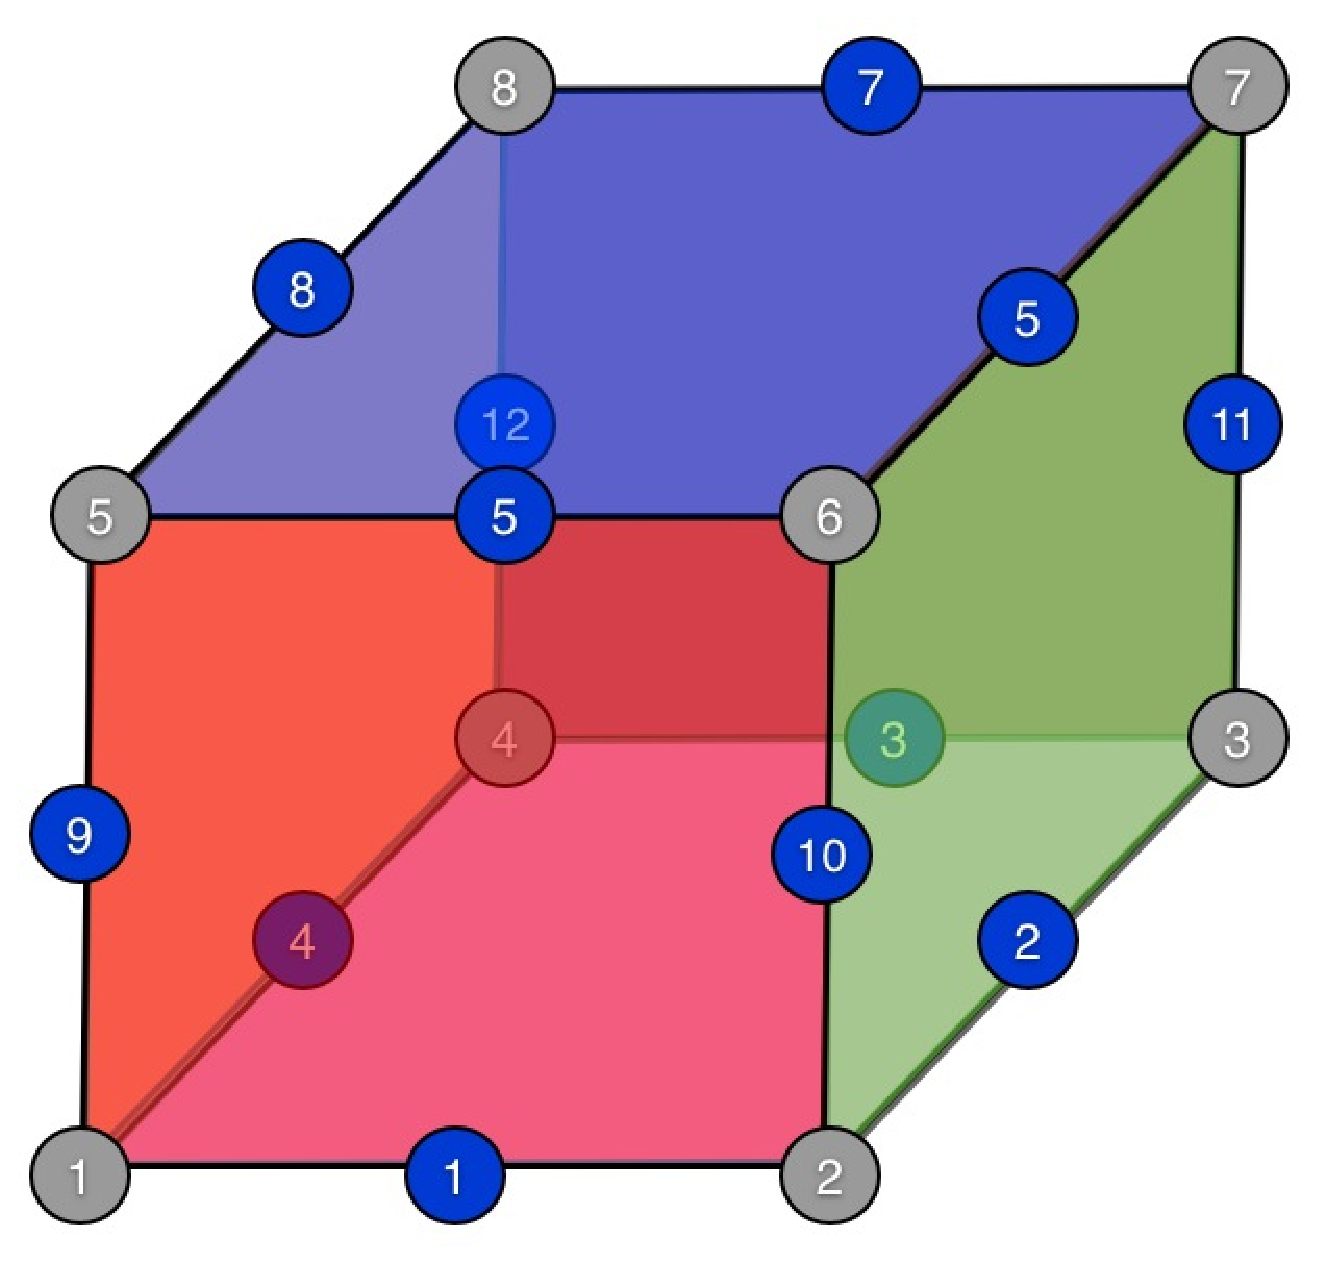
\includegraphics[width=3in]{Numbering}
\caption[8pt]{Numbering scheme for vertexes and curves.  Vertex
  numbers are in grey circles on corners, curve numbers are in blue
  circles centered on the curve.}
\label{fig:numbering}
\end{figure}

Now that we know the limitations of T3dScale, we can move on to the
special flags which must be included in the input file to have
T3dScale know what to do.  At the end of each line declaring a feature
on the bounding surfaces (vertex, curve, patch) include a comment
which reads \verb|# global| (note the space between the \# and
``global'').  T3d should be run using option \verb|-p 8| as well to
generate additional output for other file conditioners used by PFEM3d.

\subsubsection{T3d File Names}
T3dScale takes only one argument for the file name and assumes the
extensions of all the other files.  Files should be named as follows:
\begin{itemize}
\item T3d input files should be named \verb|[name].t3d|
\item T3d mesh files should be named \verb|[name].out|
\end{itemize}

\subsection{T3dScale Options and Running}
Now we have generated the mesh for one processor and it is time to
create the large, distributed computational domain.  This is done
using T3dScale.  We simply pass the program a base file name, the
number of domains to create (must be a power of two), and the
dimensions of the sub-domain (for one processor).  This is done at
run time by executing the following:
\begin{verbatim}
T3dScale -f [base file name] -xyz [space delimited dimensions] -np [number of domains]
\end{verbatim}
This will create the computational domain for the example, where every
processor has the same (give or take a few boundary nodes) number of
nodes, elements, internal features, etc.  T3dScale outputs the mesh
files for each domain named \verb|[name].out.[domain #]|, and the list
of regions and the boundary conditions for the entire domain (assumed
to be fixed on the bottom and pushed/pulled at the top) in a file
named \verb|[name].out.bc|.  The contents of these supporting files
(the BC and regions) can either be manually or automatically (via some
other script) included in the header files for PFEM3d.

\section{Summary}
Computational domains consisting of $2^n$ identical smaller
rectangular-cubic domains can be constructed using T3dScale providing
that all of the requirements such as proper numbering and flagging of
the boundary features has been done.

If any bugs are encountered in using T3dScale or this document would
be improved by any additions, please notify Matt Mosby via email at mmosby1@nd.edu

\end{document}
